\chapter{Datasets}
\label{c:datasets}

\section{Car Hacking dataset}

These datasets were generated as part of the study published by \cite{Song2020}. Traffic was collected from a Raspberry Pi connected to a real vehicle via the OBD-II port, while another Raspberry Pi was used to inject traffic. The vehicle was parked with the engine turned on throughout the data gathering process. Five datasets were produced, with an overview of the attack datasets being available on Table \ref{tab:car_hacking_dataset_overview}.

\begin{itemize}
    \item Normal: An attack-free dataset
    \item \gls{dos} attack: Packets with the ID set to 0 were injected every 0.3 ms, impairing network availability
    \item Fuzzy attack: Packets with random IDs and payloads were injected every 0.5 ms, aiming to cause vehicle malfunction
    \item Gear spoofing attack: Packets a specific ID and payload were injected every 1 ms, successfully changing the gear value on the instrument panel
    \item RPM spoofing attack: Packets a specific ID and payload were injected every 1 ms, successfully changing the RPM gauge on the instrument panel
\end{itemize}

\begin{table}
    \centering
    \begin{tabular}{*{3}{c}}
        \toprule
        \textbf{Attack type} & \textbf{Normal messages} & \textbf{Injected messages}\\
        \midrule
        DoS Attack & 3,078,250 (84\%) & 587,521 (16\%)\\
        Fuzzy Attack & 3,347,013 (87\%) & 491,847 (13\%)\\
        Gear Spoofing & 2,766,522 (82\%) & 597,252 (18\%)\\
        RPM Spoofing & 2,290,185 (78\%) & 654,897 (22\%)\\
        \bottomrule
    \end{tabular}
    \caption{Car Hacking dataset overview}
    \label{tab:car_hacking_dataset_overview}
\end{table}

\section{IEEE Car Hacking: Attack \& Defense Challenge 2020}

The datasets published by \cite{kang2021car} were created to be used in the Car Hacking: Attack \& Defense challenge. It had two rounds: preliminary and final. For the preliminary round, training and submission datasets were provided, both containing driving and stationary vehicle traffic. For the final session, a single dataset with multiple attacks was created.\par
An overview of the preliminary datasets can be seen on Table \ref{tab:ieee_challenge_dataset_overview}. For both driving and stationary scenarios, the datasets contained flooding, spoofing, replay, and fuzzing attacks. Attack-free datasets were also provided.

\begin{table}
    \centering
    \begin{tabular}{*{7}{c}}
        \toprule
        \textbf{Purpose} & \textbf{Status} & \textbf{Flood} & \textbf{Spoof} & \textbf{Replay} & \textbf{Fuzzy}\\
        \midrule
        \multirow{4}{*}{Training} & \multirow{2}{*}{Driving} & 77,373 & 3,879 & 23,775 & 45,474\\
        & & (4.1\%) & (0.2\%) & (1.3\%) & (2.4\%)\\
        & \multirow{2}{*}{Stationary} & 76,807 & 3,877 & 23,818 & 44,405\\
        & & (4.3\%) & (0.2\%) & (1.3\%) & (2.5\%)\\
        \midrule
        \multirow{4}{*}{Submission} & \multirow{2}{*}{Driving} & 96,559 & 22,489 & 37,869 & 44,770\\
        & & (4.8\%) & (1.1\%) & (1.9\%) & (2.2\%)\\
        & \multirow{2}{*}{Stationary} & 95,120 & 20,094 & 25,012 & 51,923 \\
        & & (5.4\%) & (1.1\%) & (1.4\%) & (3.0\%)\\
        \bottomrule
    \end{tabular}
    \label{tab:ieee_challenge_dataset_overview}
\end{table}

\section{Automotive Controller Area Network (CAN) Bus Intrusion Dataset v2}
\label{subsec:tue_dataset}

The datasets made available by \cite{Dupont2019} consists of bus data from an Opel Astra, a Renault Clio, and a custom built prototype. For all three systems, attack-free datasets were provided along with datasets containing diagnostic, fuzzing, replay, spoofing and \gls{dos} attacks.

\section{CrySyS Lab}
\label{sec:dataset_crysys}

This dataset was obtained from \cite{crysys} and consists of CAN traffic collected from 25 minutes of driving in the highway as well as in small streets. A variety of packet modification attacks were simulated using the tool publicly available in \cite{infector}, which allows for easy modification of CAN log files. These attacks consist of modifying the payload of packets with a given ID, akin to a man-in-the-middle attack. Five attack datasets were generated, along with the attack-free version, and the attacks target the payload of the packets with ID 120 starting at 50\% and ending at 90\% of the total file. The attacks consist of holding the payload at a constant value, modifying the payload to be a random value, adding an increasing amount to the original payload, decreasing the payload from 255 to 0 and repeating, and adding a delta of 1000 to the original payload. Unlike other datasets, were packet insertion is performed and the attack can mostly be detected via the interval between arriving packets, these attacks do not insert any packets. Attacks can only be detected by observing anomalies in the behaviour of the payloads.

\section{CES}

The setup used to generate real CAN traffic can be seen on Figure \ref{fig:setup}. It is composed of various real vehicle ECUs, along with a modern touchscreen, and a Raspberry Pi to capture CAN traffic and running the IDS here proposed. Three attacks were simulated (fuzzing, flooding, and spoofing) by inserting packets every 200ms. The following unlabelled datasets were generated:

\begin{itemize}
    \item Baseline: 2,508,370 packets of attack-free traffic.
    \item Fuzzy attack: 184,833 packets containing two instances of a fuzzing attack.
    \item Denial-of-Service attack: 235,187 packets containing two instances of a Denial-of-Service attack.
    \item Left blinker spoofing attack: 375,569 packets containing two instances of a spoofing attack targeting the left blinker signal.
\end{itemize}

\begin{figure}
    \centering
    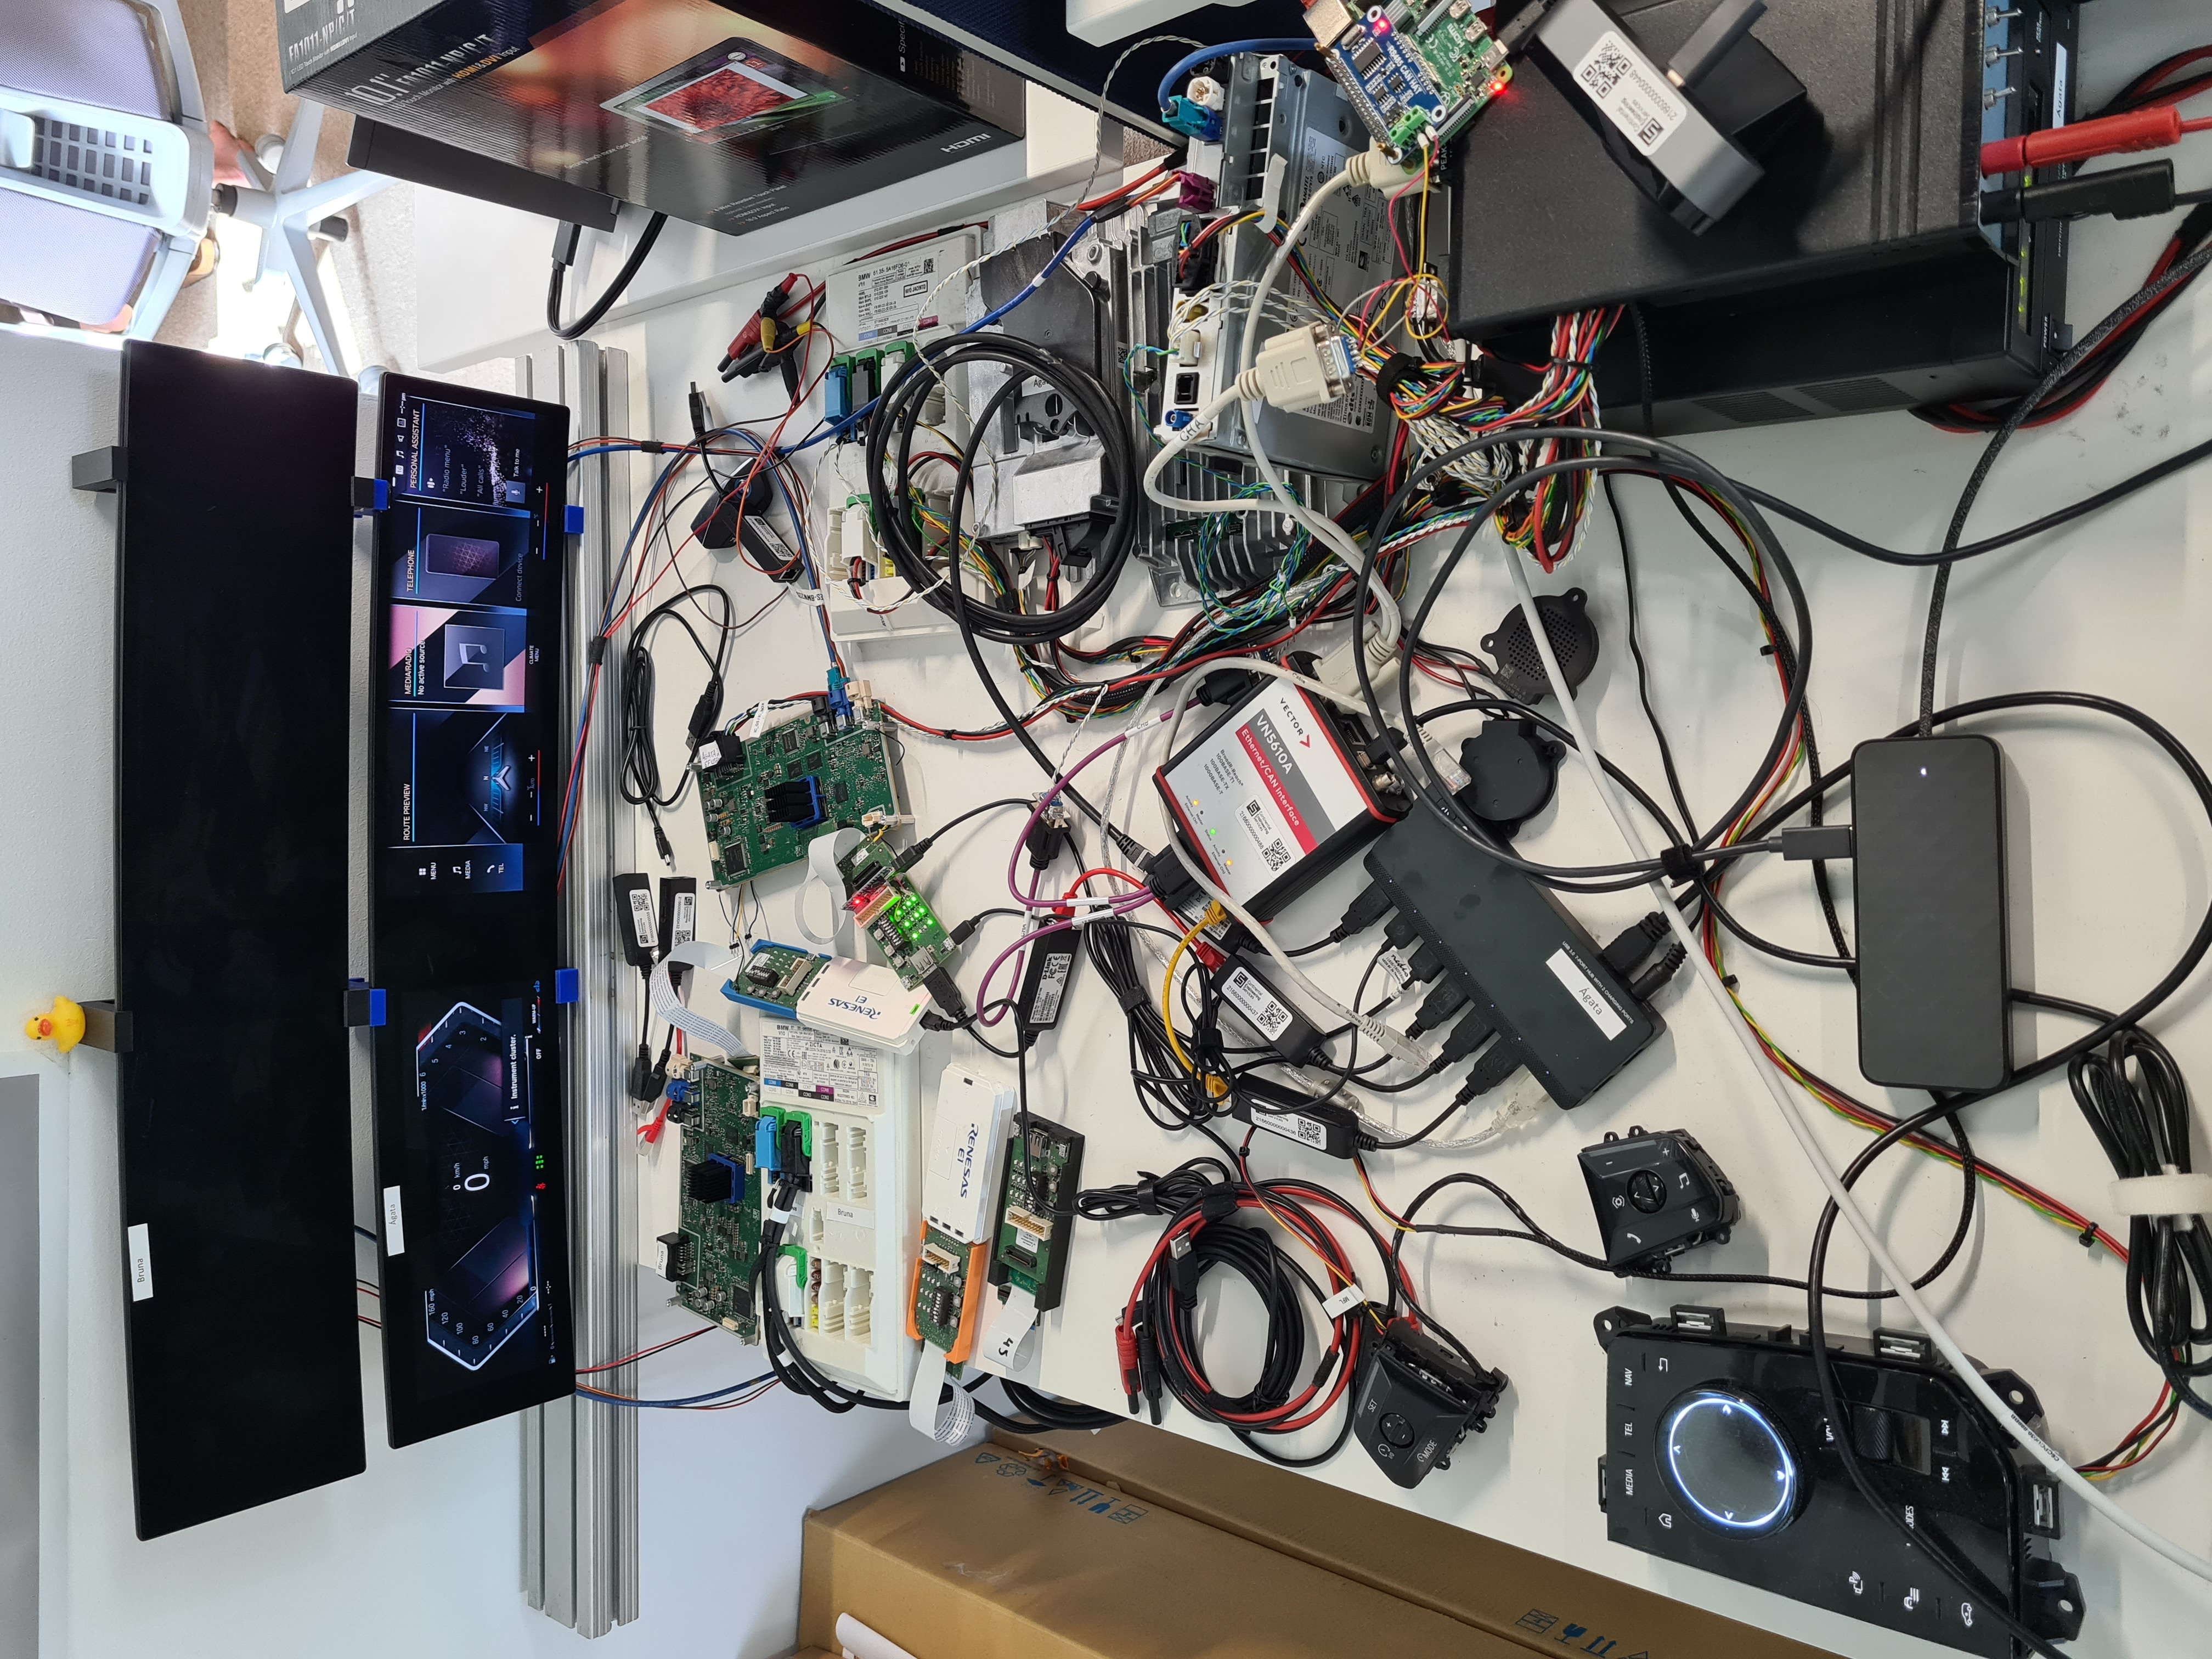
\includegraphics[angle = -90, origin = c, width = .3\linewidth]{img/parts/app/Setup.jpg}
    \caption{Setup used to generate real CAN traffic}
    \label{fig:setup}
\end{figure}